\section{Behavioral Design Pattern - Mediator}
\label{sec:mediator}

\hspace{3mm} O \textit{Design Pattern} comportamental \textit{Mediator} consiste no \textbf{desacoplamento} dos diversos componentes (objectos) entre si. Desta forma em vez de um objecto comunicar explicitamente com um outro, este fá-lo indirectamente através do \textbf{mediator}.

A implementação genérica do design pattern é a seguinte:

\begin{figure}[H]
    \centering
    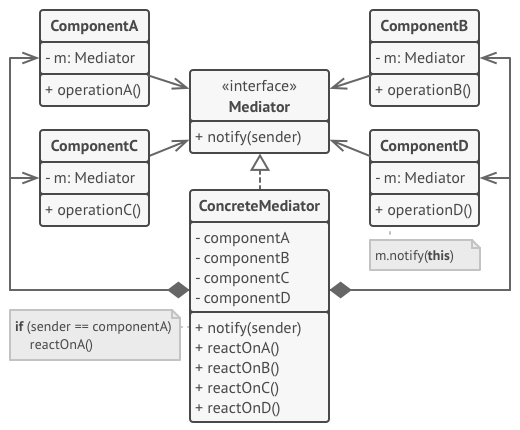
\includegraphics[scale=0.48]{images/mediator_generic_architecture.png}
    \caption{Implementação genérica do design pattern Mediator.}
    \label{fig:mediator}
\end{figure}

Partindo desta arquitectura decidiu-se implementar um exemplo em específico que consiste na gestão de componentes de uma interface gráfica, mais concretamente quando um utilizador clica num botão (Button) é obtido o seu nome, previamente introduzido numa caixa de texto de input (TextInput) e de seguida é apresentada uma mensagem de saudação - "Hello <nome>!" - numa caixa de texto de output (TextBox).

\begin{figure}[H]
    \centering
    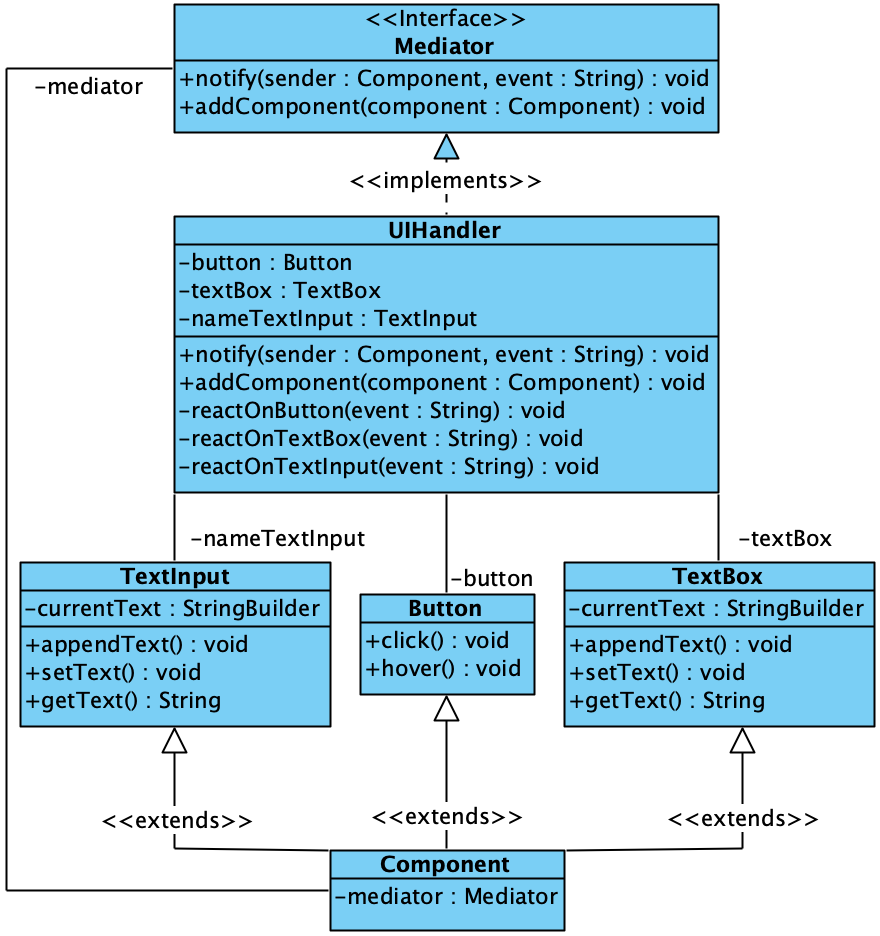
\includegraphics[scale=0.5]{images/class_diagram_mediator.png}
    \caption{Diagrama de classes da implementação.}
    \label{fig:mediator-1}
\end{figure}

A implementação mais fácil, no entanto não a mais correta, seria o botão (Button) conhecer as caixas de texto (TextInput e TextBox), desta forma quando o mesmo fosse clicado simplesmente este acedia à caixa de texto de input (TextInput) para obter o nome e depois à caixa de texto de output (TextBox) para definir a mensagem. \textbf{No entanto, só neste pequeno exemplo, o botão (Button) já tem uma dependência de 1 para 2, sendo que se o botão interagisse com N componentes diferentes essa dependência também aumentava para N}. A manutenção deste código torna-se-ia cada vez mais complicada uma vez que a alteração de um componente ou da forma como esse componente interage com outro poderia exigir a alteração de várias classes.

Uma forma de resolver este problema é a introdução de um objecto mediador (Mediator) que fica responsável pela interacção dos vários componentes entre si. Assim todos os componentes (Button, TextInput e TextBox) \textbf{dependem unicamente do mediador (Mediator), reduzindo assim as dependências de 1 para N para 1 para 1}. Da mesma forma o mediador (Mediator) tem acesso a todos os componentes.

A implementação seria da seguinte maneira, o botão (Button) notifica o mediador (Mediator) que foi clicado (event), de seguida o mediador (Mediator) acede à caixa de texto de input (TextInput) para obter o nome e depois à caixa de texto de output (TextBox) para definir a mensagem. \textbf{Note-se que apesar de se continuar com uma dependência de 1 para N no Mediator, esta dependência é apenas neste objecto}.

